This section will outline the approaches taken to develop and compare a suite of
classifier models as well as the gathering and preparation of a custom coffee
bean defect dataset.

\section{Sample gathering and dataset development}
\label{sec:sample-gathering-and-dataset-development} At the early stages of the
project, it became clear that public coffee bean image datasets will not be suitable
for the aims of this project as they often lack in variety of defects as well as
suffer from a lack of labelling in that regard.
Therefore, a custom dataset,
reflecting the variety of existing defects and coffee varieties was necessary to
ensure that any developed model can cope with the diversity of coffee available
on the market.

The gathered dataset consisted of roughly two kilograms of roasted coffee, gathered
from two small-scale coffee roasters: Harmony Roasters based in York and Vibe
With coffee based in Nottingham.
Both roasters are in the specialty coffee market
and switch their offerings frequently, allowing them to work with a variety of
coffee suppliers and species.
Both roasters mentioned performing manual quality control
after every roast session and expressed interest in the automation of this process,
echoing the research aims of the project.

Over a period of 6 weeks between november and february 2023, both roasters were asked
to keep track of any defective beans they come across and separate the defects by
the variety the coffee belonged to.
This ensured that the roasters were not
asked to spend too much of their time and could still perform their usual duties
with as little distraction as possible.
Neither roaster asked for compensation for
their work, however, samples of non-defective beans were purchased for their usual
retail price, ensuring that the research process would not take any advantage of
their time and effort.

Upon gathering the beans, the defective beans were inspected once again with each
defect separated into its own section.
The separation was done after a
consultation with the coffee roasters, who provided a verbal description of each
defect's visual characteristics.
The non-defective beans were also double-checked
for any defects in order to ensure the least amount of incorrectly labelled
samples.

To digitize the dataset, beans of each group were arranged in $5 \times 5$ grids
(where possible) and photographed using the main lens of the Pixel 7 pro smartphone.
All images were taken on a bright white background, with care taken to not include any dust or debris in the image.
Overhead lights along with a smaller tabletop light were used to make sure lighting levels stayed consistent between pictures.
Images of each defect were stored locally on the smartphone with a backup made
in google images and GitHub.

Overall, the dataset contained 2786 images, each annotated with the bean variety,
the processing method used and the defect (or lack thereof) present in the bean.
It should be noted that despite the initial aims, the distribution of defects in
the final dataset was imbalanced, with certain defects occurring much less
frequently than others.
To attempt to combat this, in cases where a bean
exhibited several defects at once, it was labelled as the rarer defect.
For
example, if the bean was both a ''quaker`` (underdeveloped) and had insect damage,
it was labelled as having insect damage only.
While not a perfect solution, this
ensured a satisfactory number of images per class.
A further description of the dataset
is provided below.

\subsection{Dataset description and statistics}
\label{subsec:dataset-description-and-statistics}
\begin{figure}[h]
	\begin{subfigure}
	{0.2\textwidth}
		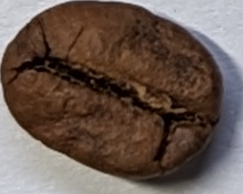
\includegraphics[height=0.8\linewidth, keepaspectratio]{
			./figures/methodology/quaker-bean
		}
		\subcaption{''Quaker``} \label{fig:quakerBeanSingle}
	\end{subfigure}
	\begin{subfigure}
	{0.2\textwidth}
		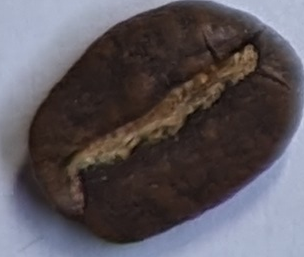
\includegraphics[height=0.8\linewidth, keepaspectratio]{
			./figures/methodology/normal-bean
		}
		\subcaption{Normal} \label{fig:normalBeanSingle}
	\end{subfigure}
	\begin{subfigure}
	{0.2\textwidth}
		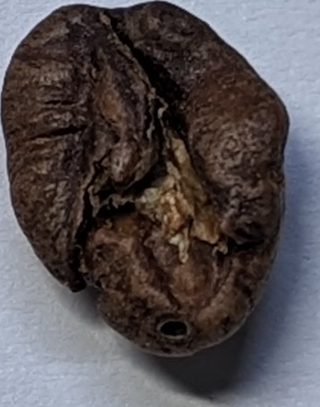
\includegraphics[height=0.8\linewidth, keepaspectratio]{
			./figures/methodology/insect-damaged-bean
		}
		\subcaption{Insect \\ damage} \label{fig:insectBeanSingle}
	\end{subfigure}
	\begin{subfigure}
	{0.2\textwidth}
		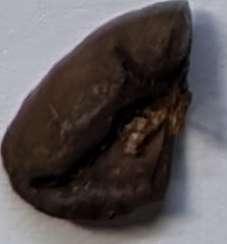
\includegraphics[height=0.8\linewidth, keepaspectratio]{
			./figures/methodology/bean-fragment
		}
		\subcaption{Bean \\ fragment} \label{fig:fragBeanSingle}
	\end{subfigure}
	\begin{subfigure}
	{0.25\textwidth}
		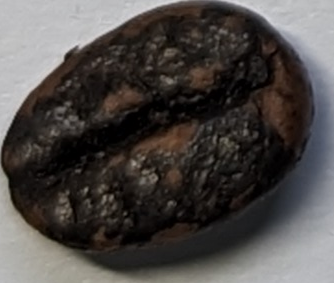
\includegraphics[height=0.8\linewidth, keepaspectratio]{
			./figures/methodology/burnt-bean
		}
		\subcaption{Burnt} \label{fig:burntBeanSingle}
	\end{subfigure}
	\begin{subfigure}
	{0.25\textwidth}
		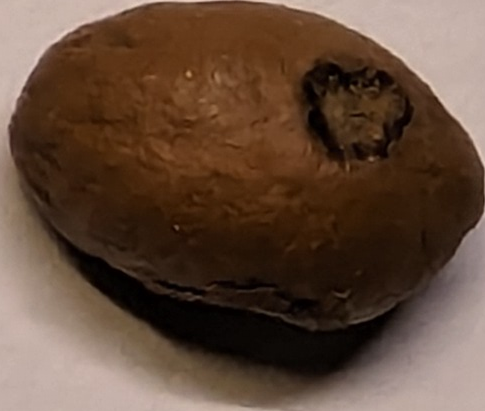
\includegraphics[height=0.8\linewidth, keepaspectratio]{
			./figures/methodology/mold-damaged-bean
		}
		\subcaption{Mould damage} \label{fig:moldBeanSingle}
	\end{subfigure}
	\begin{subfigure}
	{0.25\textwidth}
		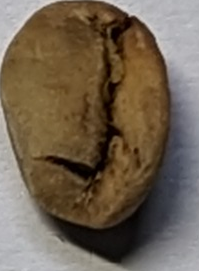
\includegraphics[height=0.8\linewidth, keepaspectratio]{
			./figures/methodology/under-bean
		}
		\subcaption{Underroasted} \label{fig:underBeanSingle}
	\end{subfigure}
	\caption{Examples of bean defects}
	\label{fig:beanDefects}
\end{figure}

Keeping in line with the project
aims, this section will mainly focus on the defects identified in the beans
contained in the dataset.
Overall, the beans exhibited five various defects, whose
counts and short descriptions are presented in table~\ref{tab:beanDefectCounts}.
Figure~\ref{fig:beanDefects} provides a brief look at the various defects, with more
examples shown in the appendix % TODO add appendix with more images

\begin{table}[h]
	\centering
	\begin{tabular}{|p{0.25\linewidth}|p{0.6\linewidth}|p{0.15\linewidth}|}
		\toprule \textbf{Defect name} & \textbf{Visual features}                                                                                                                                             & \textbf{Count} \\
		\midrule Normal bean          & Even colour, brown to dark-brown hue, no surface damage or blemishes and a round shape with no deformities                                                           & 1311           \\
		Quaker                        & Light brown to brown hue (due to less caramelisation of sugar), scorch marks, brown spots on surface.
		Occasionally, a shrivelled, uneven look of the outside surface & 978            \\
		Bean fragment                 & Significantly deformed or chipped exterior, smaller bean pieces                                                                                                      & 296            \\
		Underroasted                  & Very light brown exterior, dark green or yellow in extremely underroasted beans                                                                                      & 104            \\
		Burnt                         & Dark brown to black exterior, significant scorching or an oily, shiny surface                                                                                        & 50             \\
		Insect/mould damage           & Small, round holes or larger ''craters`` on the surface                                                                                                              & 47             \\
		\bottomrule
	\end{tabular}
	\caption{Bean defect counts}
	\label{tab:beanDefectCounts}
\end{table}

The beans in the dataset belonged to a total of nine varieties and have been processed using six different methods.
The number of beans belonging to each processing method and variety method is shown
on figures~\ref{fig:beanProcessingCounts} and~\ref{fig:beanVarietyCounts} respectively.
\begin{figure}[h]
	\centering
		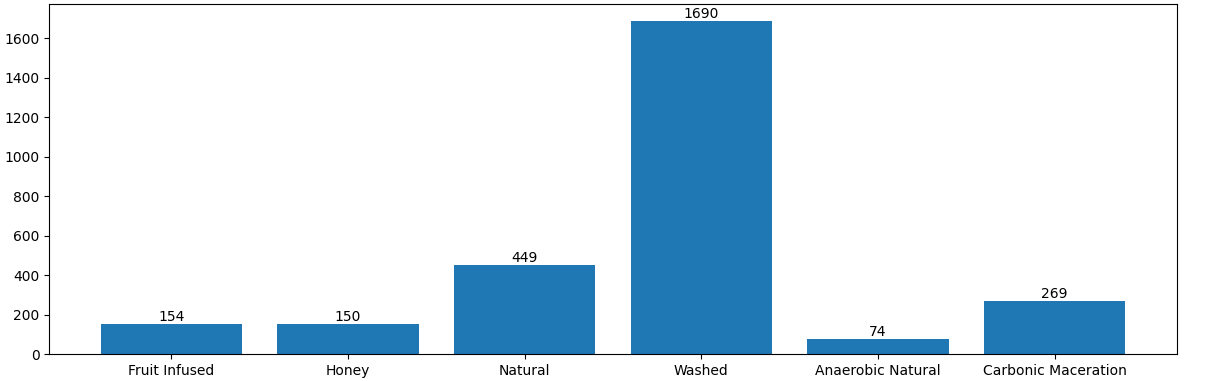
\includegraphics[width=\linewidth, height=2.5cm]{
			./figures/methodology/processing-counts
		}
	\caption{Bean processing method counts}
	\label{fig:beanProcessingCounts}

	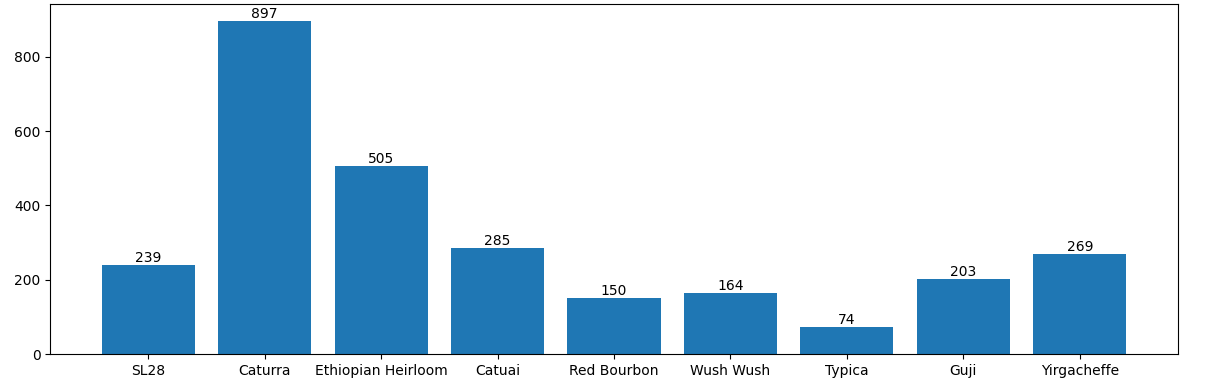
\includegraphics[width=\linewidth, height=2.5cm]{
			./figures/methodology/variety-counts
		}
	\caption{Bean variety counts}
	\label{fig:beanVarietyCounts}
\end{figure}

It should be noted that the original intent was for the insect and mould damage to be distinct classes,
however, these defects are quite rare, especially with the higher-grade green coffee the local roasters worked with.
Because of this lack of available data, it was decided to merge the classes: not only do the visual features of the two
defects resemble each other, but the effects they have on the final product are also similar.
While future work could seek an improved dataset and a higher granularity of classes, the merging of the two classes here
is unlikely to reduce the practical usefulness of the classifier in a roaster's daily tasks.
\subsection{Data pre-processing}
\label{subsec:data-pre-processing}
As described in the above section, the beans were arranged in grids when their pictures were taken.
To train the classifier however, each bean had to be contained in its own image, requiring the use of a software solution
to automatically separate each bean.
The solution was implemented in Python and depended heavily on the OpenCV library~\cite{opencvLibrary}, which provides
tools for working with and processing images.

Separating the grid images involved several steps.
First, the image was loaded and converted to grayscale using a built-in OpenCV function.
Then, a threshold was applied to the resulting images to provide a binary separation between the beans and the background.
An important step was inverting the thresholded images so that the background was represented by black pixels
and the beans by white ones - this was required for the contour finding step that followed.

Once the binary images were produced, the \verb |findContours| function was used to identify the contours and
bounding rectangles of each individual bean.
At this stage, additional checks were conducted to ensure that no dust or foreign objects were captured by the algorithm:
bounding rectangles whose areas were uncharacteristically small or large or whose aspect ratio was too imbalanced were rejected.
The expected dimensions were gathered by running the algorithm once and inspecting the produced images: the images tended
to be around 200--400 pixels wide/tall, with an aspect ratio not exceeding 1:3.
Finally, the batch images were separated into sections matching the positions and dimensions of each bounding rectangle.
The resulting images were named reflecting the bean's variety, origin, processing method and defect class and sorted into folders
named in the same pattern.
A CSV file reflecting the class annotations has also been generated and stored in the image directory.
Each row in the CSV file corresponded to a single bean, with the columns containing the image name and the
aforementioned class information.

A visualisation of the data processing pipeline is shown on figure~\ref{fig:imgProcessing}.

\begin{figure}[h]
	\centering
\begin{tikzpicture}
	\node (raw)
		{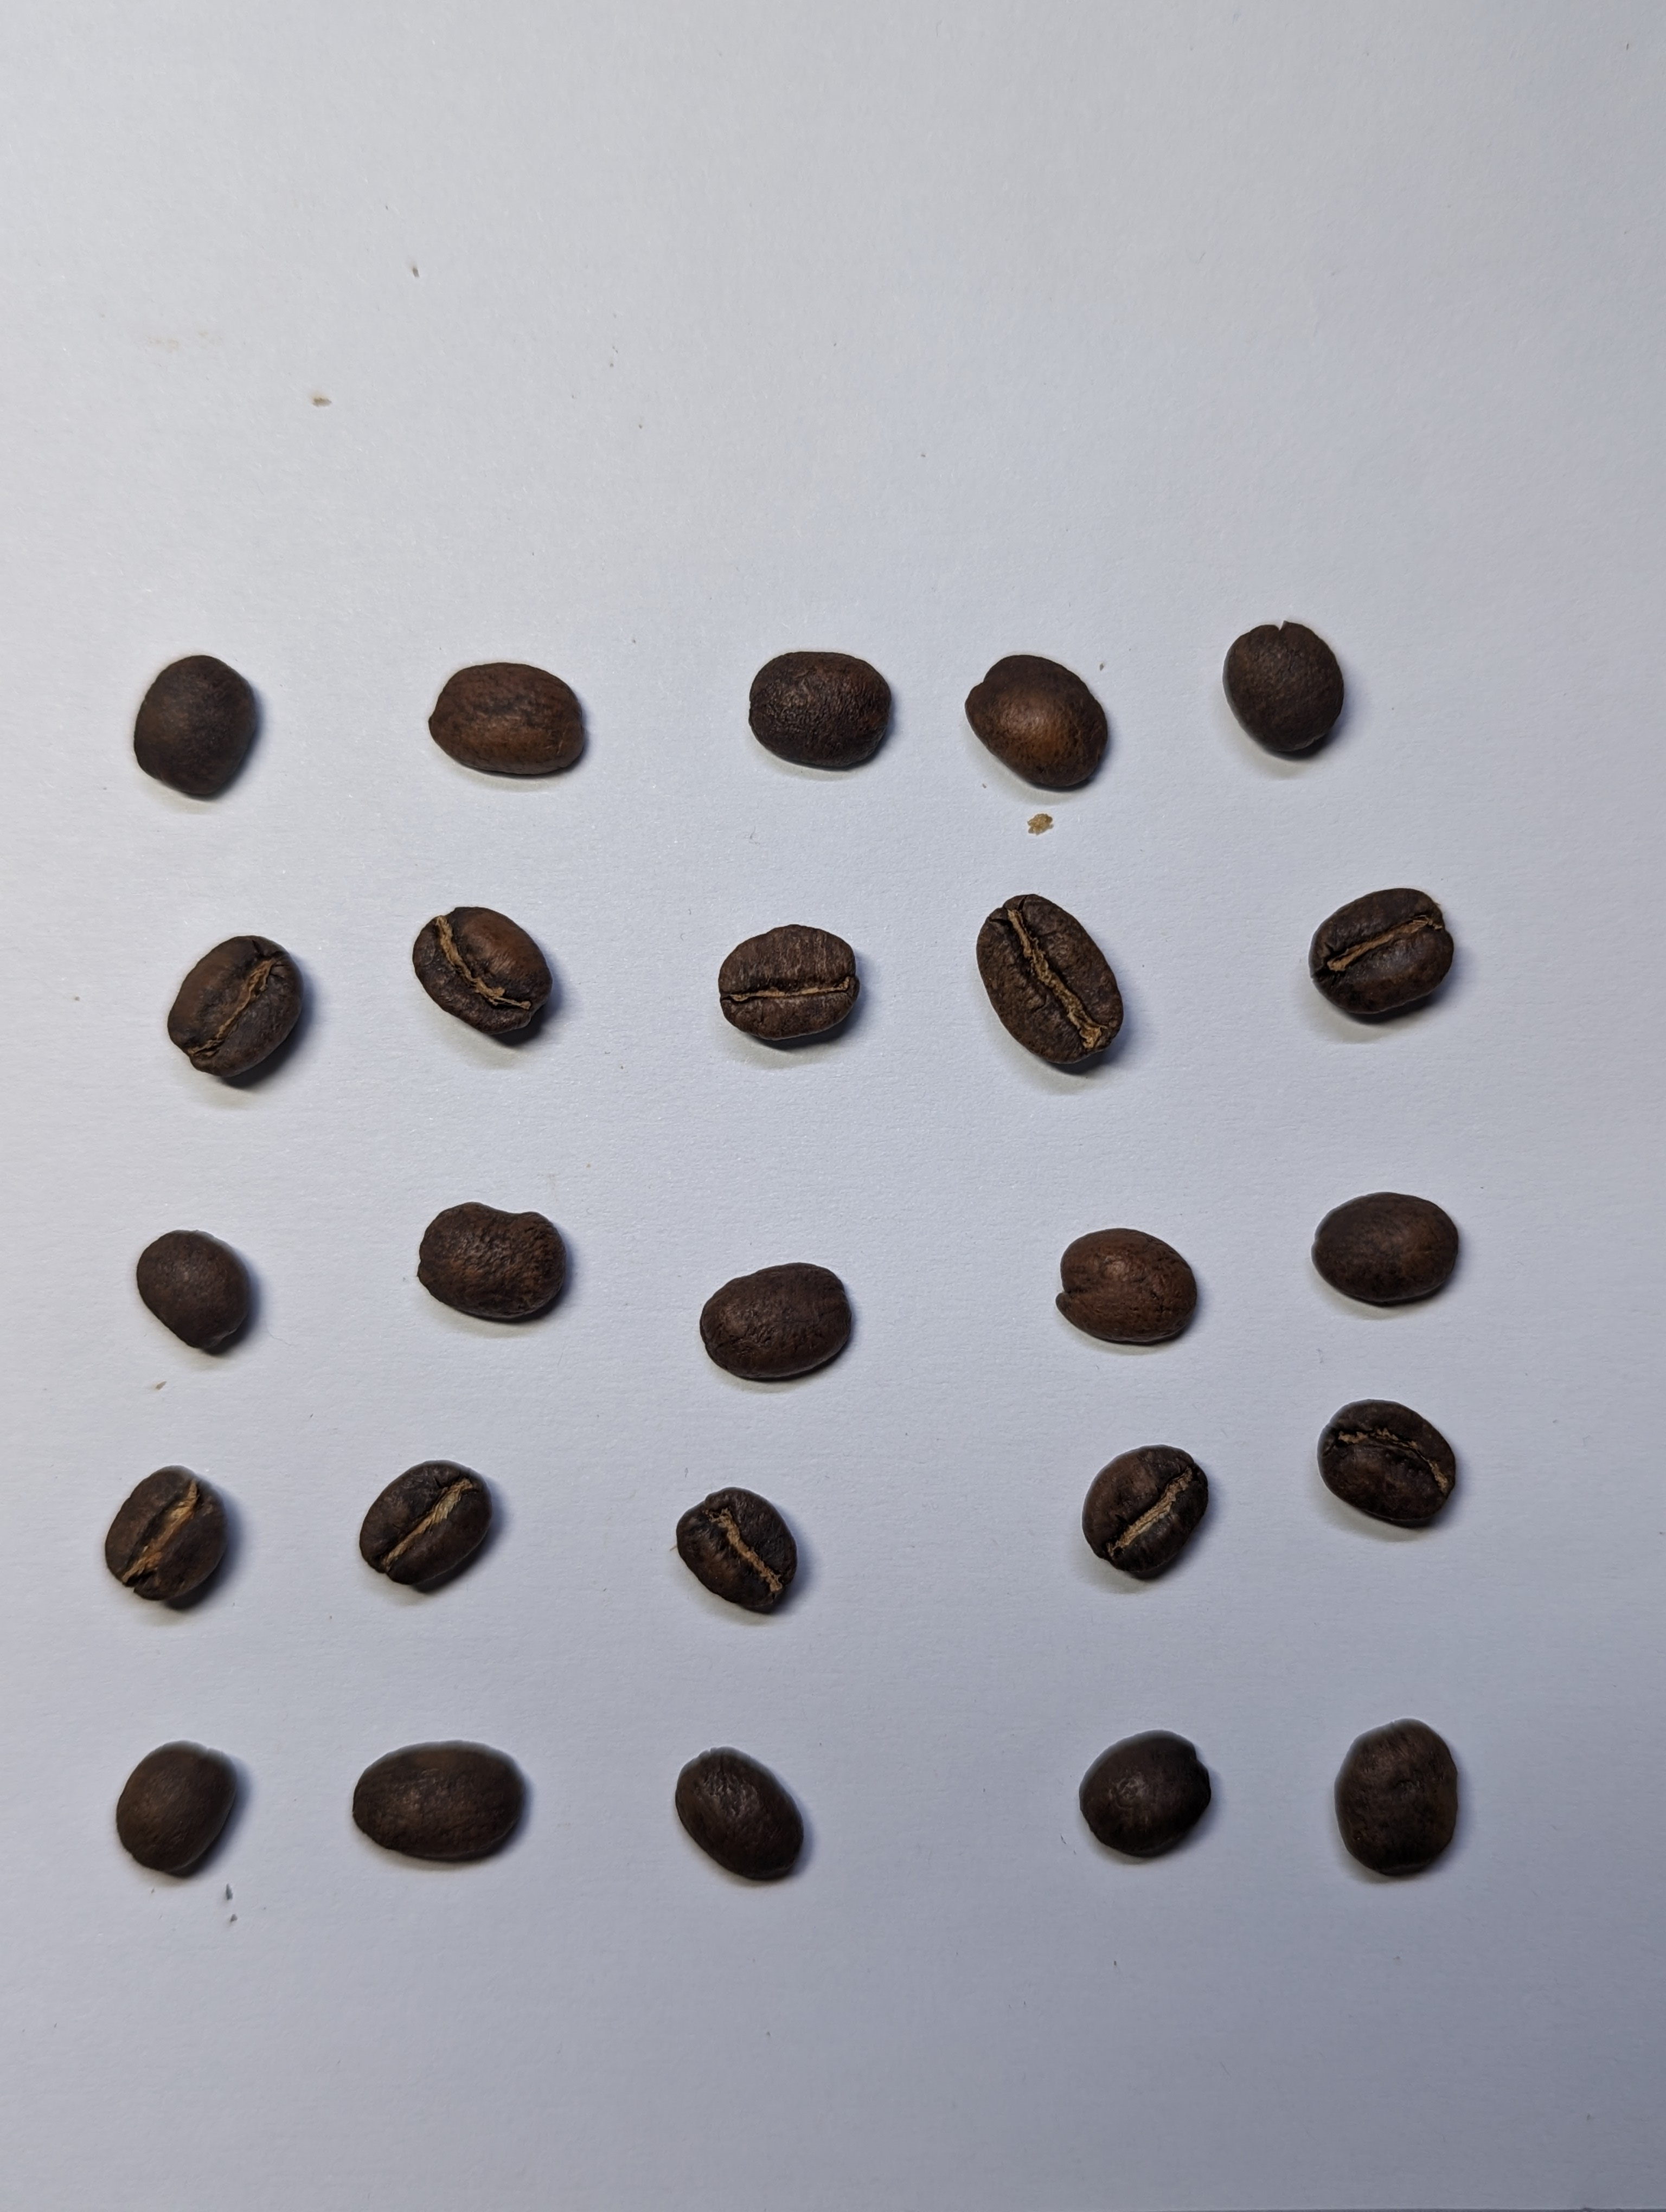
\includegraphics[height=4cm, keepaspectratio]{methodology/bean-batch-raw}};
	\node[right=of raw](gray)
		{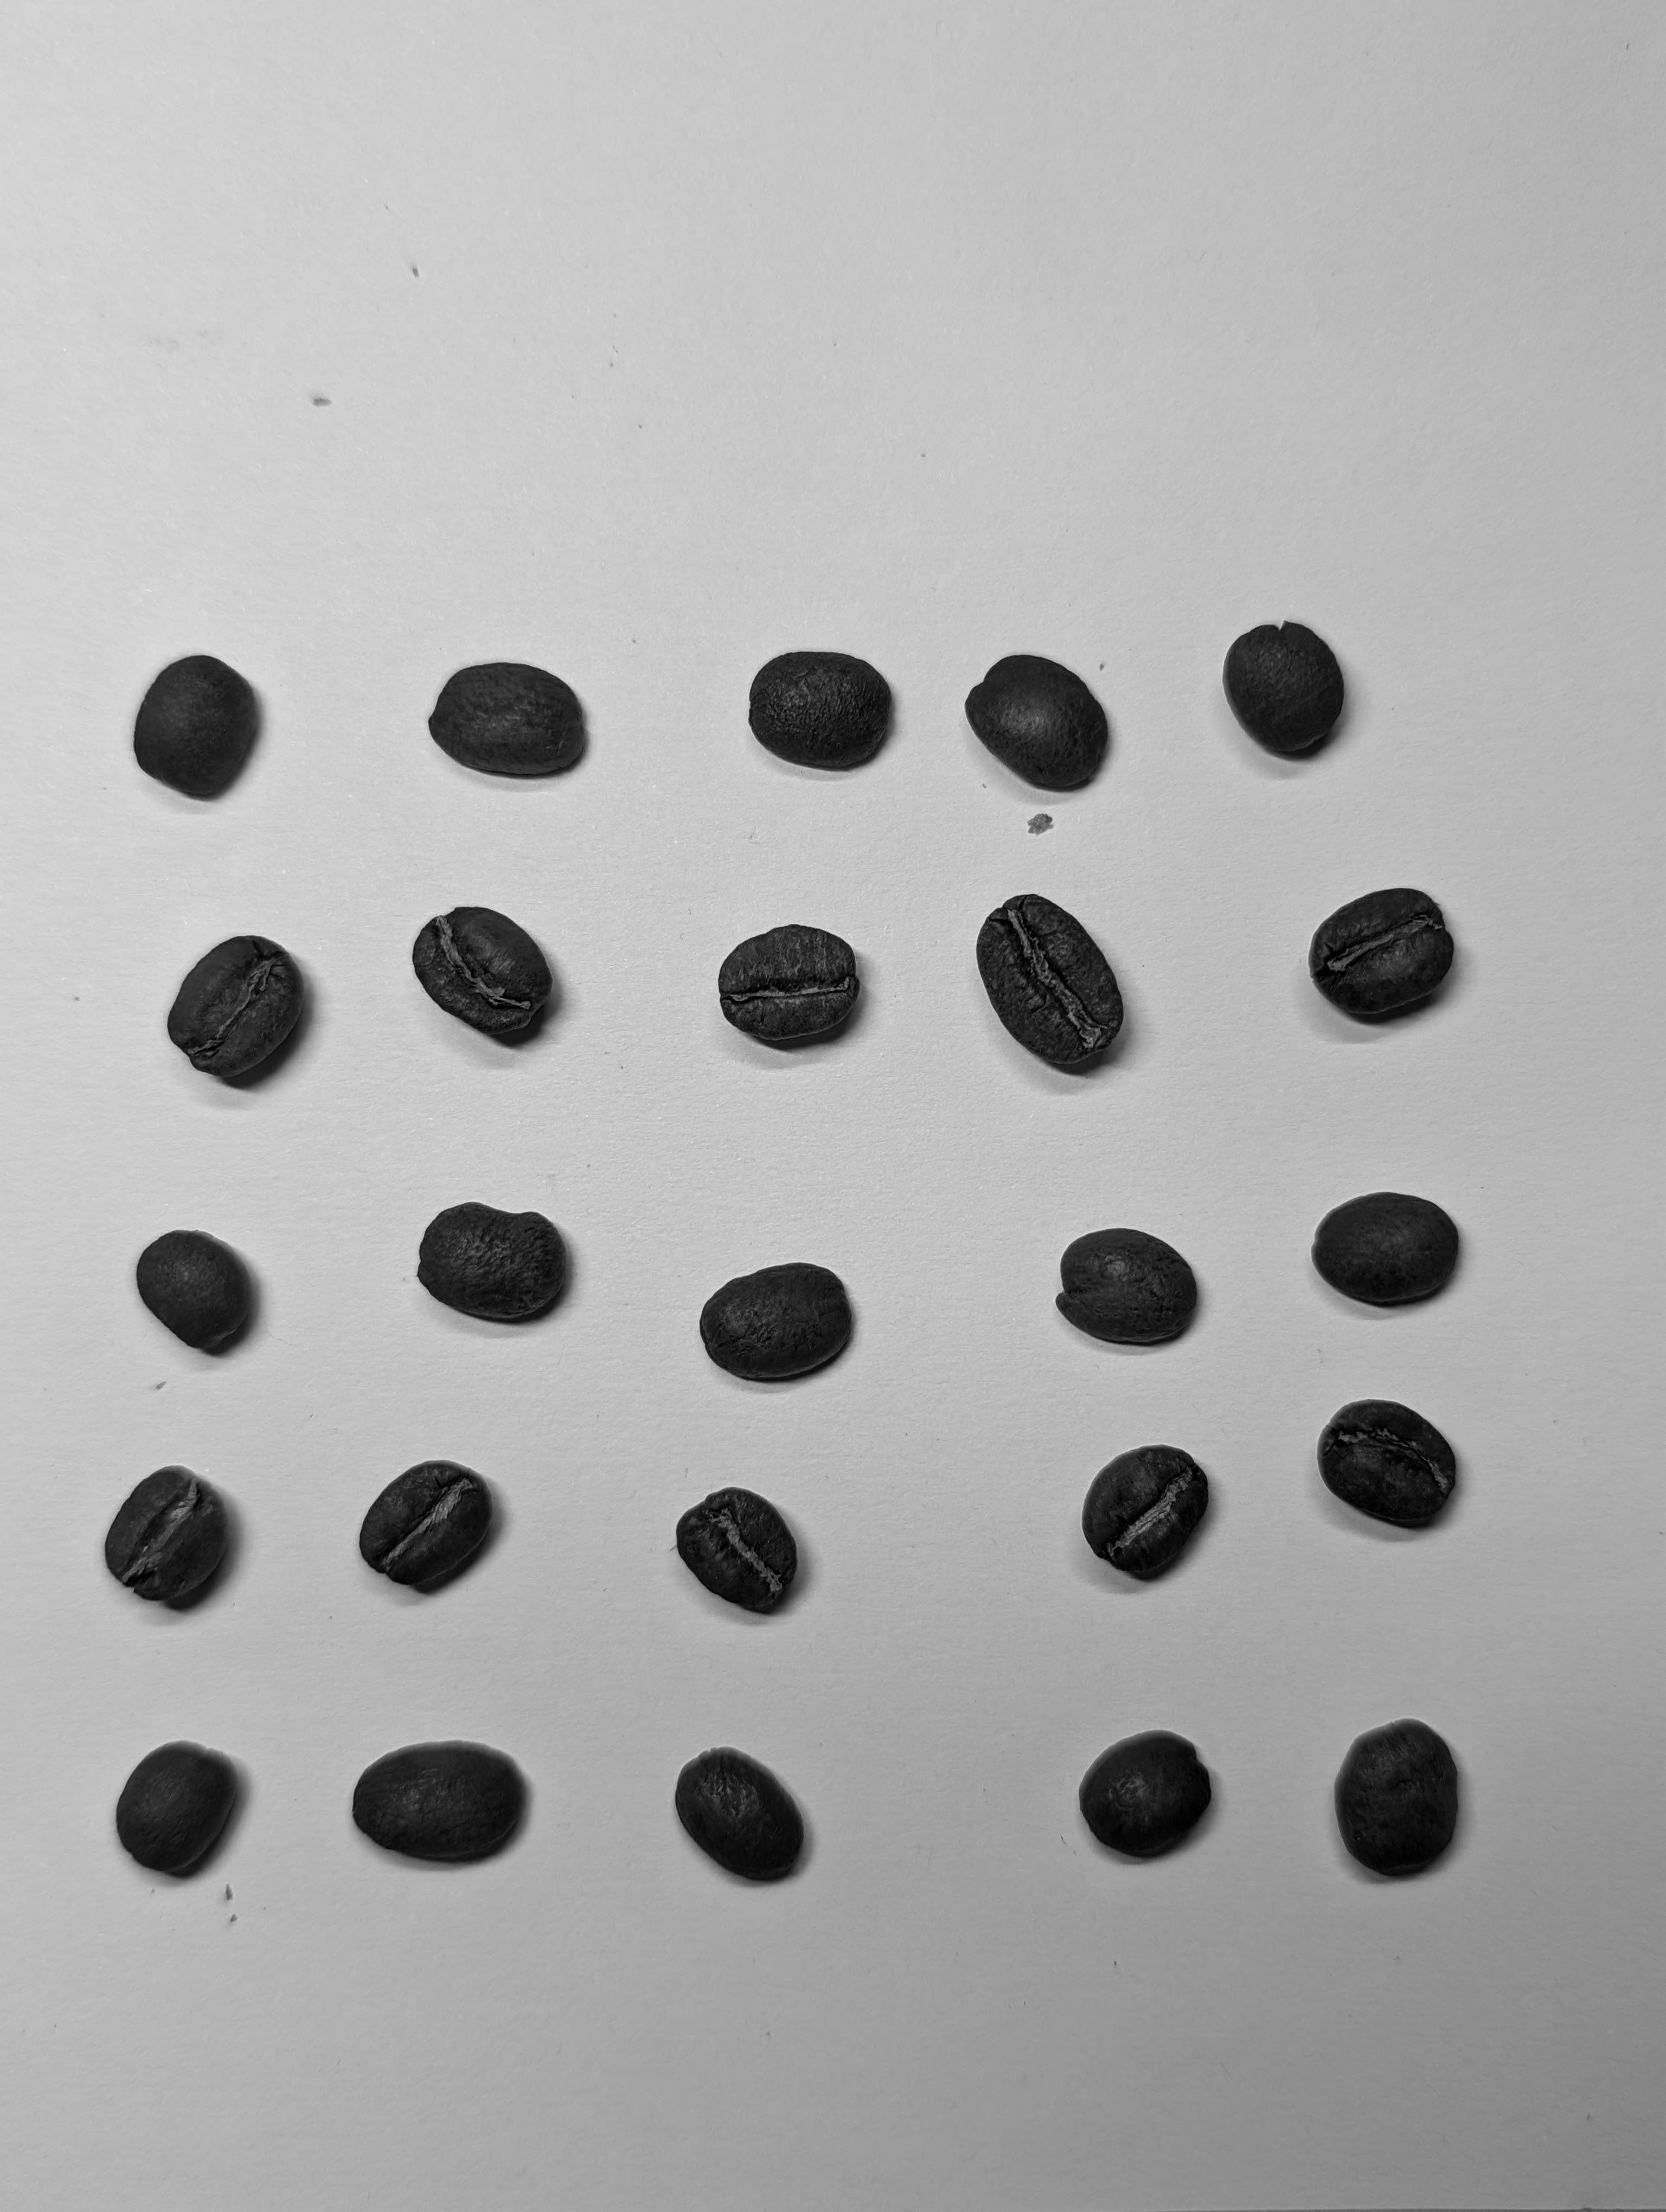
\includegraphics[height=4cm, keepaspectratio]{methodology/bean-batch-gray}};
	\node[below=of gray] (thresh)
		{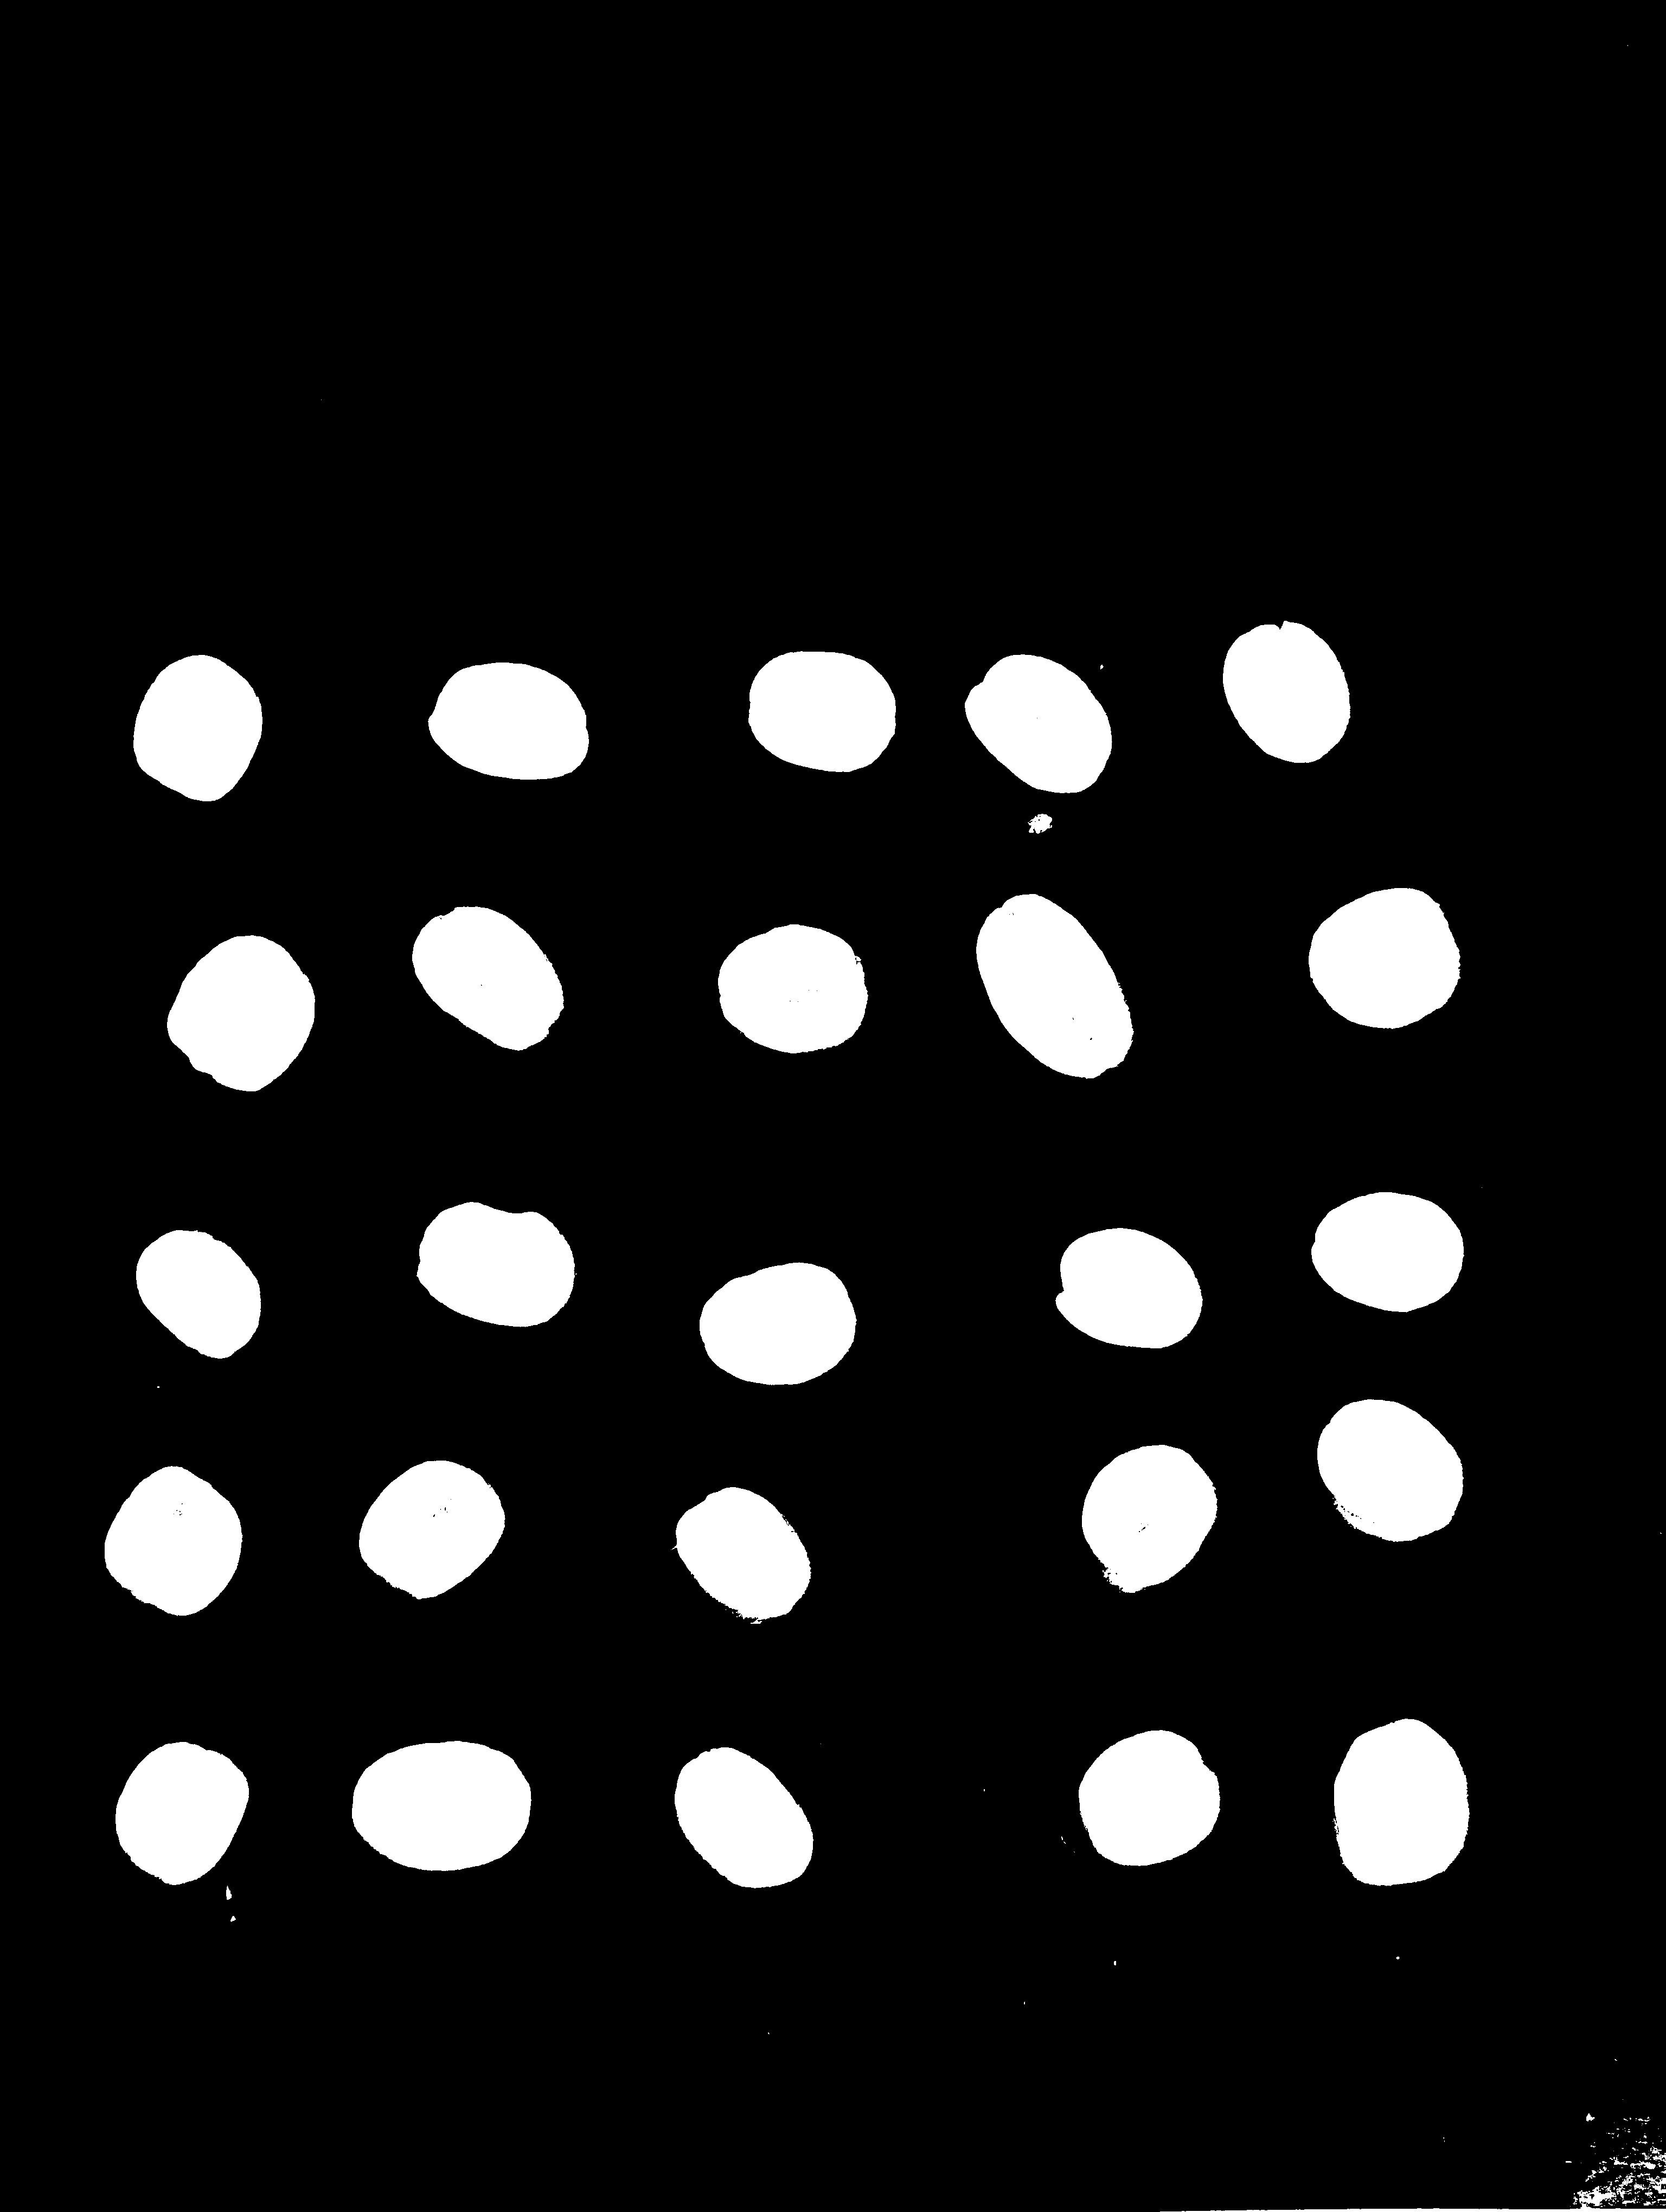
\includegraphics[height=4cm, keepaspectratio]{methodology/bean-batch-thresh}};
	\node[left=of thresh, below=of raw] (contours)
		{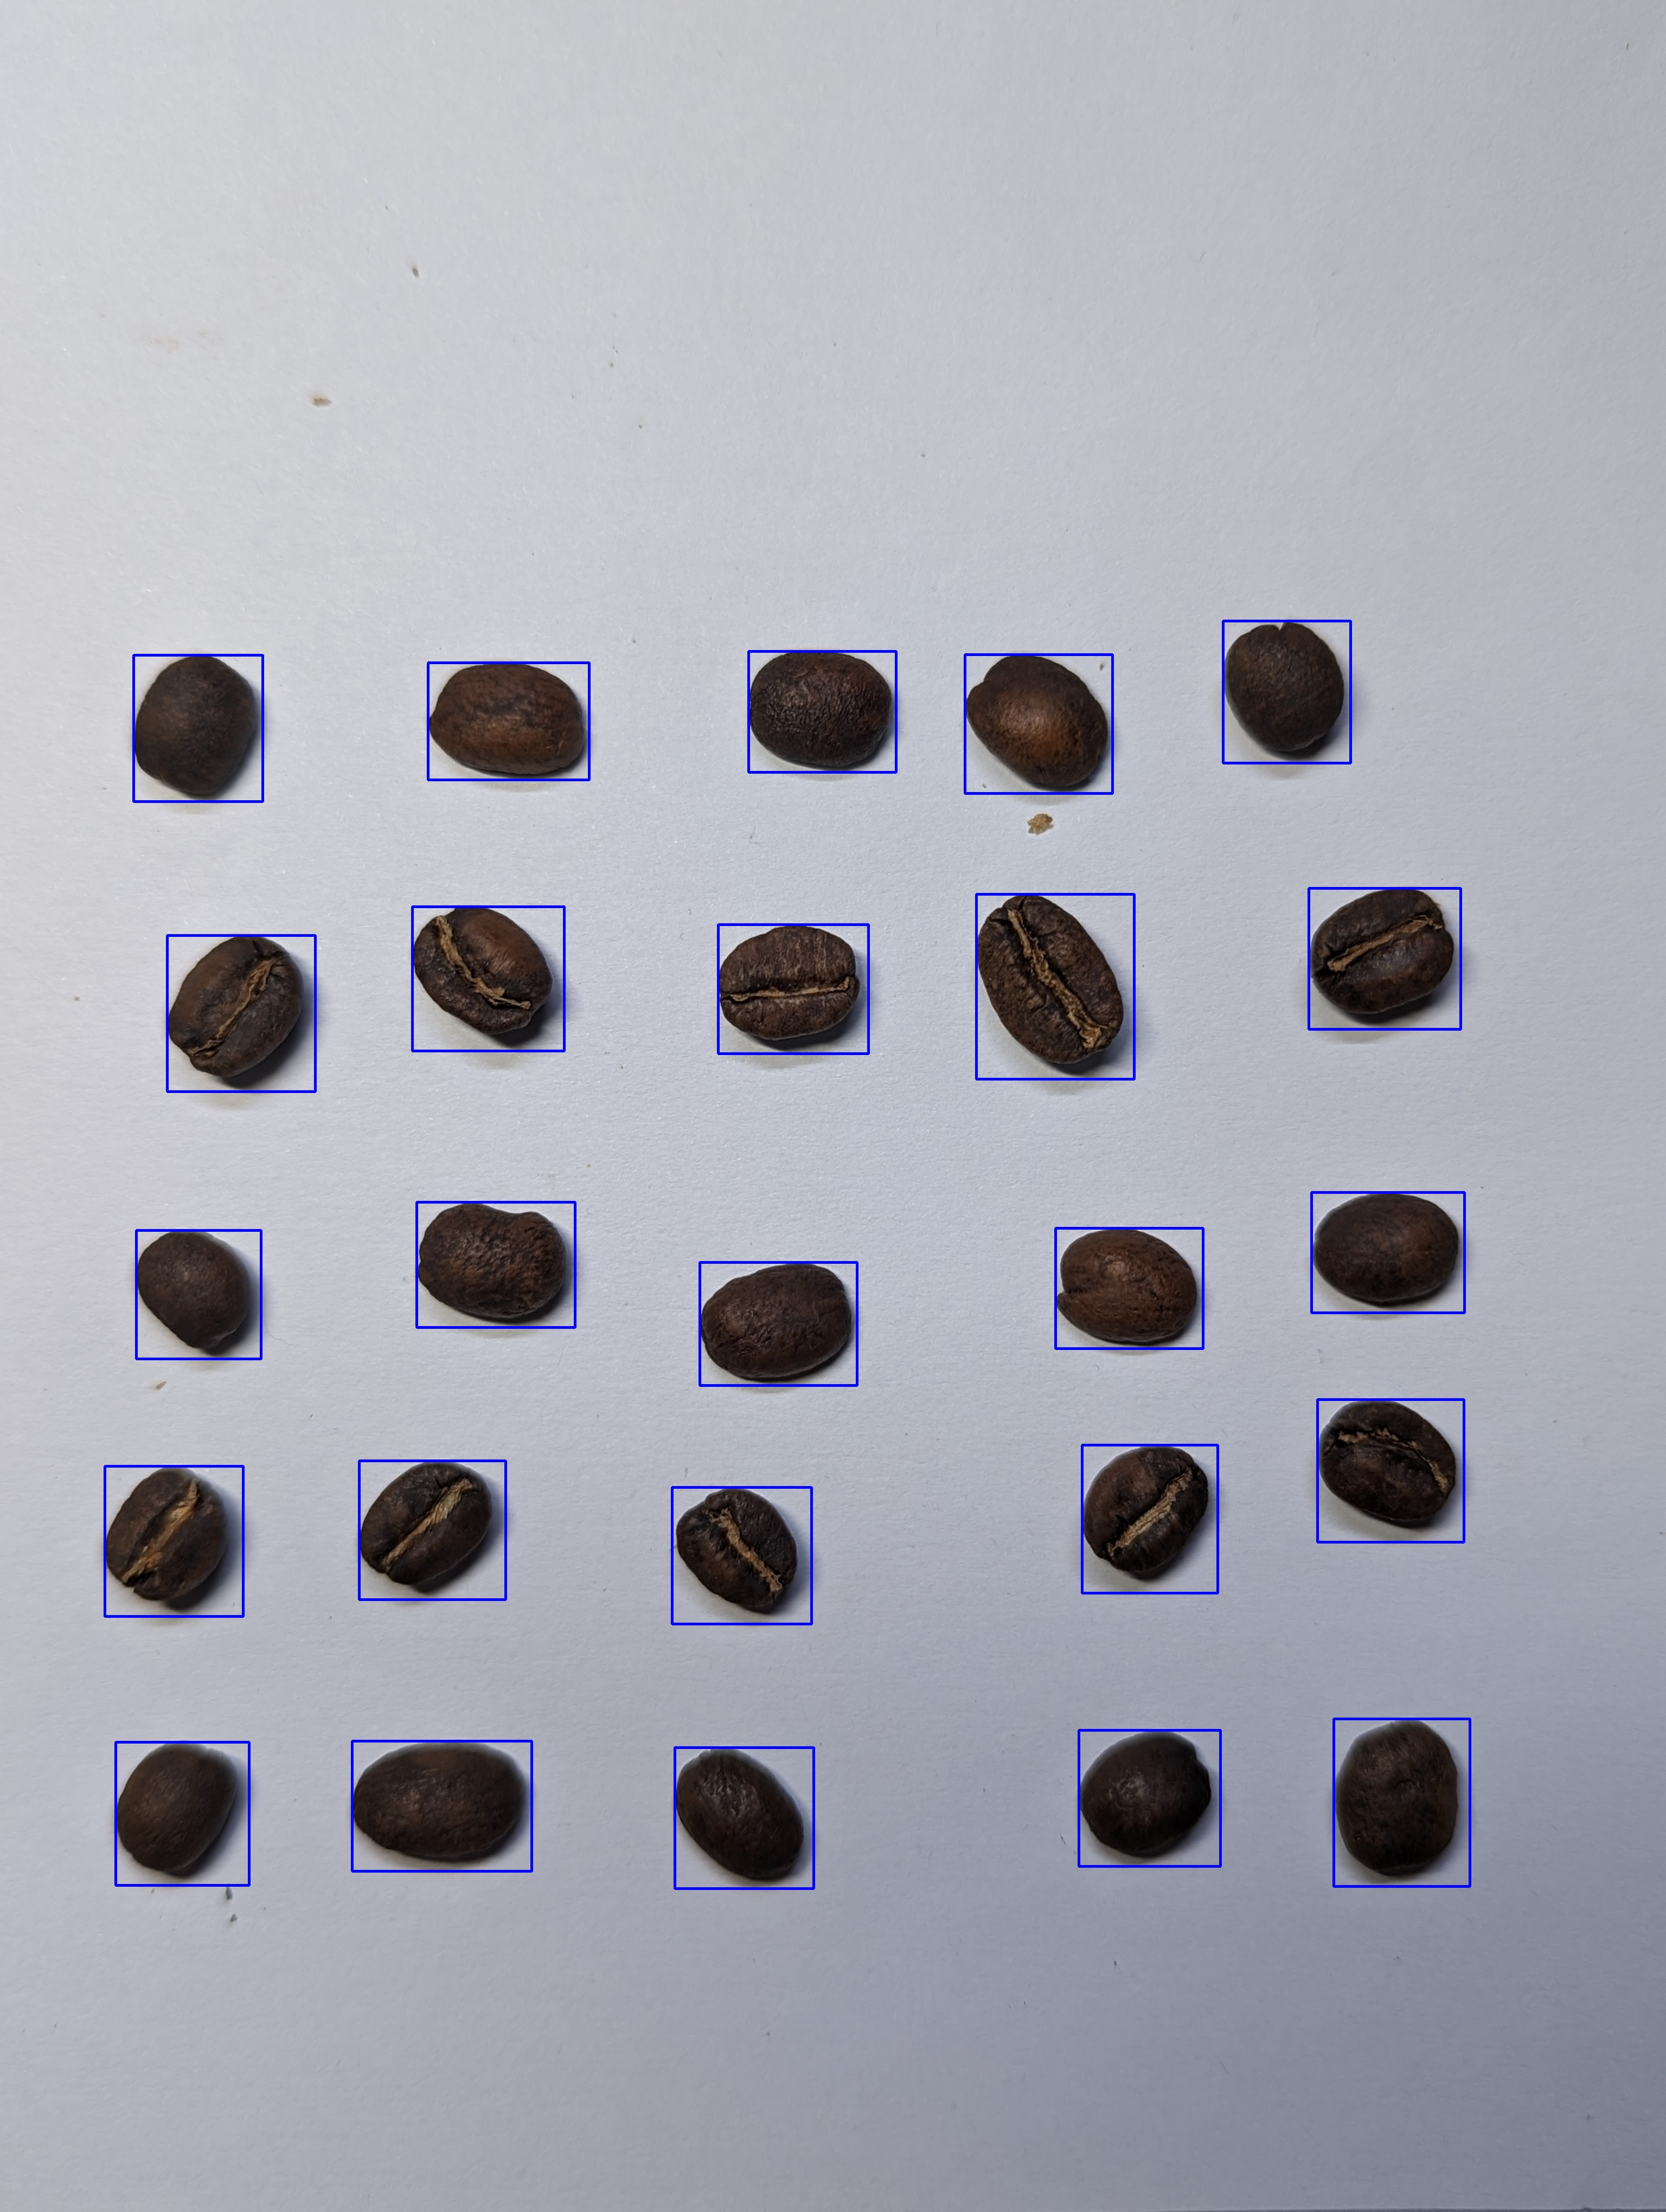
\includegraphics[height=4cm, keepaspectratio]{methodology/bean-batch-contours}};

	\draw[->,thick] (raw) -- (gray);
	\draw[->,thick] (gray) -- (thresh);
	\draw[->,thick] (thresh) -- (contours);
\end{tikzpicture}
	\caption{Image processing pipeline}
	\label{fig:imgProcessing}
\end{figure}

It should be noted that preliminary experiments led to another addition to the image processing steps:
it was found that better performance was achieved when the natural background of the images was replaced with pure white pixels.
To achieve that, the thresholded images were used to manually set all non-bean (i.e. black) pixels to a value of (255, 255, 255),
resulting in a pure white background.
Both versions of the datasets were retained and used in classifier training.

Overall, the data processing pipeline yielded a dataset containing the individual images in a nested directory, with
a CSV annotations file in the top-level directory to be used by a machine learning framework.

\section{Approaches to model development}
\label{sec:approaches-to-model-development}
The following section outlines the approaches taken in implementing a suite of image classifiers for bean defects.
The classifiers were implemented in Python, and, where applicable, were trained on an M3 Apple Silicon system with 36GB
of memory.

The literature review identified 3 general paths that one could take when developing a classifier, each with a different
set of strengths, weaknesses, and aiming to address different priorities.
The following subsection will discuss the approach taken to develop the three models to be evaluated further, in an
increasing order of complexity.
\subsection{Nearest-neighbor classifier}
\label{subsec:knn-classifier}
The primary reasoning behind implementing a KNN-based classifier is its speed of deployment, simplicity of implementation
and good accuracy potential.
As a concept, KNN can be easily understood even by non-technical stakeholders and requires little experimentation apart
from picking the value of K, determining how many ''neighbors`` each input has to be compared against.

One of the main challenges with KNN is its computational cost: the number of comparisons grows quickly with an increase
in the amount of features, dimensions and data points.
Therefore, with the dataset's images containing tens of thousands of pixels, each with three colour channels, a brute-force
approach was dismissed.

An approach seen, among others, in Olivieri et. al.'s paper~\cite{hyperspectralGreenOliveri}, is dimensionality reduction,
which aims to extract the features of the data that contribute to its difference the most.
While several dimensionality reduction techniques exist, the significant visual differences across the bean classes suggested
that the use of colour histograms could efficiently reduce the size of the data while still preserving its differences.

A colour histogram is a relatively simple plot of the distribution of colours in a given image.
A strength of this approach is its resilience to the orientations of beans in the images - the colour distribution stays
the same no matter how the bean is positioned (apart from the small discrepancies in shadows).
Furthermore, by controlling the amount of distinct colours in the histogram, the dimensionality can be easily changed to
make sure there is plenty of data to compare the images by.

It should be noted that the method is not without its criticisms: while colour makes up a significant amount of the difference
between the beans, properties like texture and shape are removed by the dimensionality reduction process.
Also, the size of the image itself can skew the distribution simply due to the difference in the numbers of pixels.

Another approach to a KNN classifier was tested in a preliminary experiment:
there, the images were converted into long vectors by extracting colour information from each channel (red, green or blue)
and concatenating the three resulting grids into a one-dimensional representation.
While this approach was able to correctly classify some images, especially those belonging to the ''normal`` and ''quaker``
classes, the performance on the smaller classes combined with the long prediction times suggested that the colour histogram
provided a better compromise between the richness of the data and the practicality of the classifier.

The best hyperparameters were found in a grid search, with different choices of the value of k, the distance metric
and nearest neighbour calculation algorithm trialed.
In every experiment, the classifier was fitted with 80\% of the data, chosen at random and evaluated on the rest of the data,
with metrics such as overall accuracy, per-class precision, recall and f1 score recorded and tracked.
To maintain a consistent ratio of beans of different types, a stratified split function has been used.

The classifiers and their evaluation were implemented using the Scikit-learn library \cite{sklearnLibrary}, with the calculation of colour
distributions provided by the Scikit-image library \cite{skImageLibrary}.
Loading the data was done by creating a \verb|DataLoader| class provided by the PyTorch library \cite{pytorchLibrary}, which allowed
for the data loading to be easily shared between this classifier and ones developed later.
\subsection{Compact CNN classifier}
\label{subsec:deep-learning}
The aims in developing this classifier were centered around addressing the weaknesses of the one described above,
namely its high prediction cost and its lack of ability to extract complex features from input images.

For this, a convolutional neural network (CNN) was selected as a design candidate, based on their
efficiency at classifying images and common use in industry.
Furthermore, the principles behind the functionality of convolution layers suggest that the high resolution of the input
images would be a benefit, with the classifier being able to extract texture and shape information from each image.

While countless network architectures exist, the goal with this classifier was ensuring the smallest possible classification time,
and, therefore, smaller designs were considered.
The MobileNet V2 architecture~\cite{mobileNet} stood out for its relatively small number of parameters and a promised ability to run even on
a mobile device.
Therefore, a high performance result from such a small architecture would result in a classifier that is able to be deployed
on any system, removing the cost barrier between coffee roasters and automatic quality control methods.
Furthermore, a smaller architecture would be faster to train on a custom dataset, providing greater flexibility.

Other smaller architectures such as ShuffleNet V2`~\cite{shuffleNet} were considered and trialled in preliminary experiments,
however, MobileNet consistently outperformed the others and was therefore selected as the final model of this type.
\subsection{Application of transfer learning to large models}
\label{subsec:transfer-learning}
The models trialled in this set of experiments were the largest in terms of the number of parameters and
architectural complexity.
The idea behind using these models was that the large number of parameters could allow them to extract even more information
from the input images and gain better performance, especially in smaller classes.

A drawback of such large modules is their need for large dataset during training, a requirement which the gathered data would
struggle to fulfil.
To overcome this limitation, a technique called transfer learning was employed.
In this technique, the model is first trained on a large, not necessarily domain-specific dataset and then
''fine-tuned`` on a smaller selection of domain-specific data.
This technique allows the models to learn to extract features from images and then sharpen that knowledge by training on a dataset
specific to the given task.

A commonly used general-purpose dataset is ImageNet~\cite{imageNet}, containing over a million images belonging to a thousand
classes.
Pre-trained models were loaded from the \verb|torchvision.models| package provided by PyTorch~\cite{pytorchLibrary}.

One of the more promising architectures was ResNet~\cite{resNet}, with a deep architecture boasting a high top-1 accuracy on the imageNet dataset.
Several versions of the ResNet architecture exist, with the 18, 34 and 50 layer versions trialled in the experiments.

Other tested architectures included the EfficientNet V2~\cite{efficientNet} and the Swin transformer~\cite{swinTransformer},
which were selected for their reported accuracy on the imageNet dataset.

An important step in this set of experiments was the readjusting of the model before making predictions on the bean dataset:
since all models were tailored to ImageNet, the number of output neurons in their final fully-connected layers was mismatched.
The fixes involved inspecting the models' architectures, identifying the attribute name of the final layer, and replacing it with an
instance of the \verb|torch.nn.Linear()| class, where the number of input neurons matched that of the old fully connected layer,
and the number of outputs was equal to the number of classes in the dataset.